% ------------------------------------------------------------------
%  Figura: Flujo Model Router v2 — 3 niveles (slide 13)
%  Compilar:  pdflatex 13_router.tex
% ------------------------------------------------------------------
\documentclass[tikz, border=0.2cm]{standalone}
\usepackage[utf8]{inputenc}
\usepackage[T1]{fontenc}
\usepackage{libertine}
\usepackage{amssymb}
\usepackage{xcolor}

\definecolor{primary}{HTML}{280091}
\definecolor{secondary}{HTML}{4C5CC5}
\definecolor{accent}{HTML}{3FCFD5}
\definecolor{exgreen}{HTML}{00B299}
\definecolor{darkgray}{RGB}{80,80,80}

\begin{document}
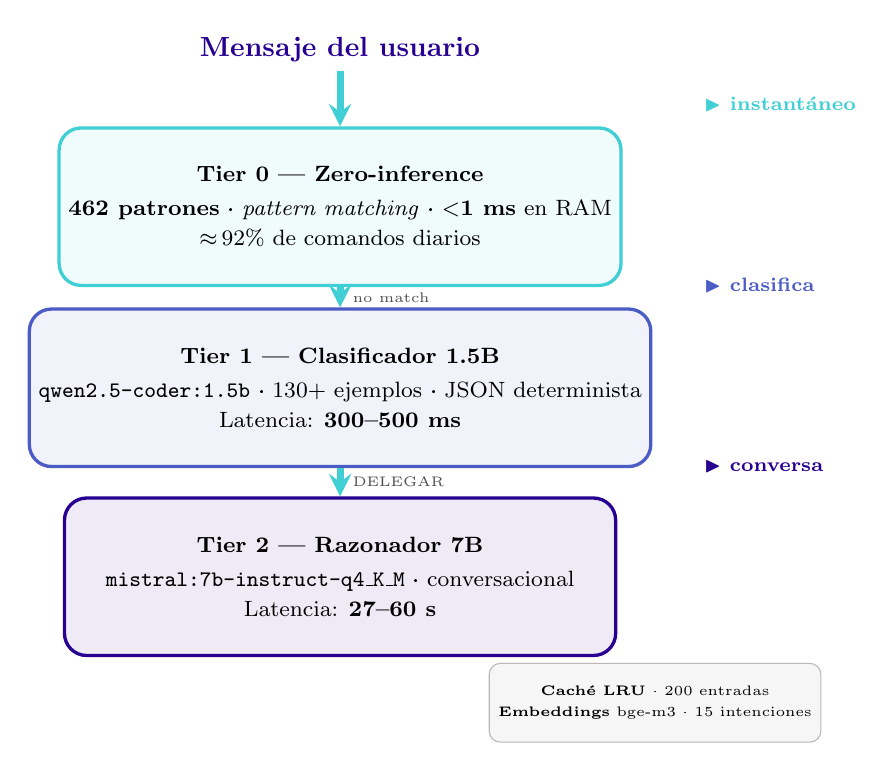
\begin{tikzpicture}[
    tier/.style={draw=#1, fill=#1!8, rounded corners=8pt,
                 minimum width=7cm, minimum height=2cm, align=center,
                 font=\footnotesize, line width=1.2pt},
    arrow/.style={draw=accent, line width=2.5pt, ->, >=stealth},
    label/.style={font=\scriptsize\bfseries\color{#1}},
]

% Entrada
\node[font=\normalsize\bfseries, text=primary] (msg) at (0, 5.5) {Mensaje del usuario};

% Tier 0
\node[tier=accent] (t0) at (0, 3.5) {
    \textbf{Tier 0 — Zero-inference}\\[0.1cm]
    \textbf{462 patrones} · \textit{pattern matching} · \textbf{$<$1 ms} en RAM\\[0.05cm]
    $\approx$\,92\% de comandos diarios
};

% Tier 1
\node[tier=secondary] (t1) at (0, 1.2) {
    \textbf{Tier 1 — Clasificador 1.5B}\\[0.1cm]
    \texttt{qwen2.5-coder:1.5b} · 130+ ejemplos · JSON determinista\\[0.05cm]
    Latencia: \textbf{300--500 ms}
};

% Tier 2
\node[tier=primary] (t2) at (0, -1.2) {
    \textbf{Tier 2 — Razonador 7B}\\[0.1cm]
    \texttt{mistral:7b-instruct-q4\_K\_M} · conversacional\\[0.05cm]
    Latencia: \textbf{27--60 s}
};

% Flechas
\draw[arrow] (msg) -- (t0);
\draw[arrow] (t0) -- (t1) node[midway, right, font=\tiny\color{darkgray}] {no match};
\draw[arrow] (t1) -- (t2) node[midway, right, font=\tiny\color{darkgray}] {DELEGAR};

% Etiquetas
\node[label=accent, anchor=west] at (4.5, 4.8) {$\blacktriangleright$ instantáneo};
\node[label=secondary, anchor=west] at (4.5, 2.5) {$\blacktriangleright$ clasifica};
\node[label=primary, anchor=west] at (4.5, 0.2)  {$\blacktriangleright$ conversa};

% Caché
\node[draw=darkgray!40, fill=darkgray!5, rounded corners=4pt,
      minimum width=3.5cm, minimum height=1cm, align=center, font=\tiny]
      at (4, -2.8) {
      \textbf{Caché LRU} · 200 entradas\\[0.05cm]
      \textbf{Embeddings} bge-m3 · 15 intenciones
};

\end{tikzpicture}
\end{document}
